% ------------------------------------------------------------------------------
% TYPO3 CMS 7.0 - What's New - Chapter "Introducción" (Spanish Version)
%
% @author	Michael Schams <schams.net>
% @author	Michel Mix <mmix@autistici.org>
% @license	Creative Commons BY-NC-SA 3.0
% @link		http://typo3.org/download/release-notes/whats-new/
% @language	Spanish
% ------------------------------------------------------------------------------
% LTXE-CHAPTER-UID:		829c5e86-1c091260-17ee2d7a-7373759a
% LTXE-CHAPTER-NAME:	Introducción
% ------------------------------------------------------------------------------

\section{Introducción}
\begin{frame}[fragile]
	\frametitle{Introducción}

	\begin{center}\huge{Introducción}\end{center}
	\begin{center}\huge{\color{typo3darkgrey}\textbf{Los hechos}}\end{center}

\end{frame}

% ------------------------------------------------------------------------------
% LTXE-SLIDE-START
% LTXE-SLIDE-UID:		a18cf273-4a7a5fcd-93de2e53-8ae1a186
% LTXE-SLIDE-ORIGIN:	c0dd5662-b64f5b3d-ea39556c-dca19b07 English
% LTXE-SLIDE-TITLE:		TYPO3 CMS 7.0 - Los hechos
% ------------------------------------------------------------------------------

\begin{frame}[fragile]
	\frametitle{Introducción}
	\framesubtitle{TYPO3 CMS 7.0 - Los hechos}

	\begin{itemize}
		\item Fecha de lanzamiento: 2 de diciembre de 2014
		\item Tipo de lanzamiento: "Lanzamiento Sprint"
		\item Visión: Abarcar. Innovar. Entregar.
		\item Enfoque principal: revisión de backend
	\end{itemize}

	\begin{figure}
		
\includegraphics[width=0.95\linewidth]{typo3-seven-zero-banner.png}
	\end{figure}

\end{frame}

% ------------------------------------------------------------------------------
% LTXE-SLIDE-START
% LTXE-SLIDE-UID:		af86d9b0-7d2f5353-e13086c0-60872995
% LTXE-SLIDE-ORIGIN:	f0c768bc-7a7f5fff-20ca5059-23f8e843 English
% LTXE-SLIDE-TITLE:		Requisitos del Sistema
% ------------------------------------------------------------------------------

\begin{frame}[fragile]
	\frametitle{Introducción}
	\framesubtitle{Requisitos del Sistema}

	\begin{itemize}
		\item PHP*:\tabto{2.2cm}v5.5.0 - v5.6.x
		\item MySQL:\tabto{2.2cm}v5.5.x - v5.6.x (no modo estricto)
		\item Espacio de disco:\tabto{2.2cm}min 200 MB
		\item Ajustes de PHP:

			\begin{itemize}
				\item memory\_limit >= 128M
				\item max\_execution\_time >= 240s
				\item opción de compilación \texttt{--disable-ipv6} \underline{no} debe ser usada
			\end{itemize}

		\item Backend requiere IE >= 9 o cualquier otro navegador moderno

	\end{itemize}

	\vspace{1cm}
	*) Detalles adicionales: \href{http://typo3.org/news/article/php-minimum-requirements-for-typo3-cms-7/}{Requisitos mínimos de PHP para TYPO3 CMS 7}

\end{frame}

% ------------------------------------------------------------------------------
% LTXE-SLIDE-START
% LTXE-SLIDE-UID:		c9664ed4-6ab76c8c-e1c5c628-3321fbc1
% LTXE-SLIDE-ORIGIN:	e6dd8a1b-2b60f76b-adc1d788-f77036d9 English
% LTXE-SLIDE-TITLE:		Línea de tiempo de lanzamiento y desarrollo
% ------------------------------------------------------------------------------

\begin{frame}[fragile]
	\frametitle{Introducción}
	\framesubtitle{Línea de tiempo de lanzamiento y desarrollo}

	\begin{figure}
		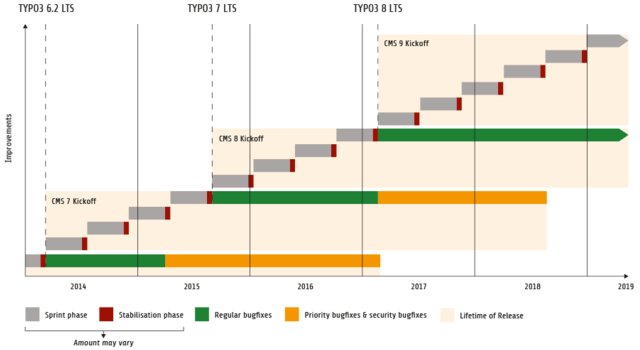
\includegraphics[width=0.90\linewidth]{Introduction/ReleaseAgenda.png}
	\end{figure}

\end{frame}

% ------------------------------------------------------------------------------
% LTXE-SLIDE-START
% LTXE-SLIDE-UID:		02a74b07-6a0d48a5-378ae469-69b98be7
% LTXE-SLIDE-ORIGIN:	a99cfec1-0a35c0fb-e552ac34-e4e407f8 English
% LTXE-SLIDE-TITLE:		Hoja de ruta de TYPO3 CMS
% ------------------------------------------------------------------------------
% https://typo3.org/typo3-cms/roadmap/

\begin{frame}[fragile]
	\frametitle{Introducción}
	\framesubtitle{Hoja de ruta de TYPO3 CMS}

	Fechas de lanzamiento estimadas y sus enfoques principales:

	\begin{itemize}
		\item
			\begingroup
				\color{typo3orange}
					v7.0 \textrightarrow\tabto{1.3cm}02/Dec/2014\tabto{3.4cm}Revisión de Backend Vol 1
			\endgroup

		\item v7.1 \textrightarrow\tabto{1.3cm}17/Feb/2015\tabto{3.4cm}Optimización \& limpieza del núcleo
		\item v7.2 \textrightarrow\tabto{1.3cm}10/Mar/2015\tabto{3.4cm}Frontend
		\item v7.3 \textrightarrow\tabto{1.3cm}21/Abr/2015\tabto{3.4cm}Ecosistema Compositor
		\item v7.4 \textrightarrow\tabto{1.3cm}09/Jun/2015\tabto{3.4cm}Revisión de Backend Vol 2
		\item v7.5 \textrightarrow\tabto{1.3cm}28/Jul/2015\tabto{3.4cm}\textit{(a ser determinado...)}
		\item v7.6 \textrightarrow\tabto{1.3cm}13/Oct/2015\tabto{3.4cm}pre-LTS inferno
		\item v7.7 \textrightarrow\tabto{1.3cm}xx/xxx/2015\tabto{3.4cm}\textbf{TYPO3 CMS 7 LTS} (Lanzamiento a largo plazo)
	\end{itemize}

	\smaller
		\url{https://typo3.org/typo3-cms/roadmap/}\newline
		\url{http://typo3.org/news/article/embrace-and-innovate-typo3-cms-7/}
	\normalsize

\end{frame}

% ------------------------------------------------------------------------------
% LTXE-SLIDE-START
% LTXE-SLIDE-UID:		d3f915ab-12d6d171-eb3858d5-12107948
% LTXE-SLIDE-ORIGIN:	185b2d64-63cab652-fa469322-8a16b1b7 English
% LTXE-SLIDE-TITLE:		Instalación
% LTXE-SLIDE-REFERENCE:	https://forge.typo3.org/issues/62578
% ------------------------------------------------------------------------------

\begin{frame}[fragile]
	\frametitle{Introducción}
	\framesubtitle{Instalación}

	\begin{itemize}
		\item Procedimiento de instalación oficial bajo Linux/Mac OS X\newline
			(DocumentRoot por ejemplo \texttt{/var/www/site/htdocs}):
		\begin{lstlisting}
			$ cd /var/www/site
			$ wget --content-disposition get.typo3.org/7.0
			$ tar xzf typo3_src-7.0.0.tar.gz
			$ cd htdocs
			$ ln -s ../typo3_src-7.0.0 typo3_src
			$ ln -s typo3_src/index.php
			$ ln -s typo3_src/typo3
			$ touch FIRST_INSTALL
		\end{lstlisting}

		\item Enlaces simbólicos bajo Microsoft Windows:

			\begin{itemize}
				\item Use \texttt{junction} bajo Windows XP/2000
				\item Use \texttt{mlink} bajo Windows Vista y Windows 7
			\end{itemize}

	\end{itemize}
\end{frame}

% ------------------------------------------------------------------------------
% LTXE-SLIDE-START
% LTXE-SLIDE-UID:		8baa2144-5611d24e-cc72d1b3-0934b840
% LTXE-SLIDE-ORIGIN:	d884c8cf-25261e85-a2a26fcd-8a64a9cb English
% LTXE-SLIDE-TITLE:		Upgrade to TYPO3 CMS 7
% LTXE-SLIDE-REFERENCE:	https://forge.typo3.org/issues/62578
% ------------------------------------------------------------------------------

\begin{frame}[fragile]
	\frametitle{Introducción}
	\framesubtitle{Actualice a TYPO3 CMS 7.x}

	\begin{itemize}
		\item Actualizaciones sólo posibles desde TYPO3 CMS 6.2 LTS
		\item TYPO3 CMS < 6.2 deberá ser actualizado a TYPO3 CMS 6.2 LTS primero
	\end{itemize}

	\begin{itemize}

		\item Instrucciones de actualización:\newline
			\smaller\url{http://wiki.typo3.org/Upgrade#Upgrading_to_7.0}\normalsize
		\item Guía oficial de TYPO3 "Instalación y actualización de TYPO3":
			\smaller\url{http://docs.typo3.org/typo3cms/InstallationGuide}\normalsize
		\item Enfoque general:
			\begin{itemize}
				\item Revisar los requisitos de sistema mínimos \small(PHP, MySQL, etc.)
				\item Revisar \textbf{deprecation\_*.log} en instancia antigua de TYPO3
				\item Actualizar todas las extensiones a las últimas versiones
				\item Desplegar fuentes nuevas y ejecutar:\newline
					Herramienta de Instalación \textrightarrow Asistente de Revisión
				\item Actualizar el módulo de inicio para usuarios backend (opcionalmente)
			\end{itemize}
	\end{itemize}

\end{frame}

% ------------------------------------------------------------------------------
